

\section{The Logic of Variable Sets}
We now give an account of the logic of variable sets as outlined in \cite{goldblatt} and by so doing present another approach to the topos semantics of $\mathcal{G}_3$.   \newline\newline


Informally speaking, in the \emph{classical} world the truth of a statement $\phi(x)$ regarding some \emph{thing} $x$ determines once and for all a set $\{x: \phi(x)\}$ of all things of which the statement is true. \newline
However, in the \emph{non-classical} world the truth-value of a statement is not \emph{absolute} but rather, \emph{context-dependent}. \newline As we saw in the Introduction varies according to the states of knowledge at some particular time. Similarly as we did before, we say that $\phi$ determines for each state $p$ a set $\phi_p$ of all the things of which the statement is known to be true at $p$ called the \emph{extension} of $\phi$ at $p$. 

\begin{definition}[$\phi_p$]
	The extension of $\phi$ at $p$ is denoted by: \begin{equation*}
		\phi_p := \{x: \phi(x)\textit{ is known at p to be true}\}.
	\end{equation*}
\end{definition}

We also require, as we saw for Kripke Semantics, that what is known now to be true remain true in the future, i.e., that truth \emph{persist} in time. 

Formalizing this construction:

\begin{definition}[$F: \textbf{P} \rightarrow \mathbb{Set}$]
	Given a frame \textbf{P} seen as a pre-order category, the assignments $p \mapsto \phi_p$ and $p \rightarrow q $ $\mapsto$ $\phi_p \subseteq \phi_q$: 
	\begin{gather*}
		\phi_p := \{x: \phi(x)\textit{ is known at p to be true}\}. \\
		\text{If } p \sqsubseteq q \text{ then } \phi_p \subseteq \phi_q
	\end{gather*}
	yield a functor $F : \textbf{P} \rightarrow \mathbb{Set}$.
\end{definition}

The category $\mathbb{Set}^\textbf{P}$ has as objects these functors which can be seen as the \emph{variable sets} $\{ \phi_p \}_{p \in \textbf{P}}$, i.e., the \emph{extensions} of $\phi$ at each stage.
\newline
The remarkable result about this category is:
\begin{prop}
	$\mathbb{Set}^\textbf{P}$  is a topos. 
\end{prop}
	This comes from a more general fact:
	\begin{thm}
		For any \emph{small} category $\mathcal{C}$ the (functor) \emph{category of diagrams} $\mathbb{Set}^\mathcal{C}$ is a topos. 
	\end{thm}
	

	In chapter 3 (\ref{examples}) we saw a few instances of this category first with $\textbf{P}= \mathbf{2} = 0 \xrightarrow{\leq_0} 1$, i.e., \emph{functions between sets} and secondly with $\textbf{P}= \mathbf{\omega} = 0 \xrightarrow{\leq_0} 1 \xrightarrow{\leq_1} 2 \xrightarrow{\leq_2}...$, i.e., \emph{sets through time}.



\newpage
\subsection{Back to Kripke Frames}

When we introduced a Kripke Frame $\textbf{P}$ as a finite poset $(P, \sqsubseteq)$ of \emph{possible worlds}, we constructed $\textbf{P}^+$ the collection of \emph{up-sets}, a.k.a. \emph{hereditary sub-sets} of the Frame and found out it could be made a Heyting algebra. \newline
Having fixed a Frame, we focus on \emph{principal} up-sets :

\begin{definition}[principal up-set]
	The principal up-set generated by an element $p \in \textbf{P}$ is:
	\begin{equation*}
		[p) := \{q : p \sqsubseteq q\}.
	\end{equation*}
	, i.e., the elements of the Frame \emph{above} $p$ in the ordering $\sqsubseteq$.
\end{definition}

The operations introduced to make  $\textbf{P}^+$ a Heyting algebra can now be characterized as:

\begin{lem} For any $S,T \in \textbf{P}^+$:
	\begin{gather*}
		S \Rightarrow T = \{p : S \cap [p) \subseteq T\}. \\
		\neg S = \{p: [p) \cap S = \emptyset\}.
	\end{gather*}
\end{lem}

If we restrict $\sqsubseteq$ to $[p)$, we can talk about the \emph{principal set generated by an element}
$q \in [p)$ denoted by $[q)_p$:

\begin{definition}
	$[q)_p := [p) \cap [q)$.
\end{definition}

More generally if $S \subseteq P$ we can \emph{relativize} $S$ to $[p)$:

\begin{definition}
	$S_p := S \cap [p)$.
\end{definition}


What we can obtain of particular interest is:

\begin{prop}
	The poset $([p)^+, \subseteq)$ of up-sets of $[p)$ ordered by inclusion forms a \emph{sub-directly irreducible} Heyting algebra with the operations defined for any up-sets $S,T \subseteq [p)$:
	\begin{gather*}
		S \cap_p T := S \cap T. \\
		S \cup_p T := S \cup T. \\
		S \Rightarrow_p T := \{q: q \in [p) \text{ and } S \cap [q)_p \subseteq T\}. \\
		\neg_p S := \{q: q \in [p) \text{ and } [q)_p \cap S = \emptyset\}.
	\end{gather*}
\end{prop} 

The notable result is that:

	If we start from an up-set $S \subseteq P$ we may choose to first relativize $S$ to $[p)$ and then apply the operations of the H.A.\footnote{H.A. stands for Heyting algebra.}  $([p)^+, \subseteq)$ or first apply the corresponding operations of the H.A. $\textbf{P}^+$ and then relativize to obtain the same result. 
	
Formally:	
\begin{lem}
	for any $S,T \in \textbf{P}^+$,
	\begin{gather*}
		(S_p) \cap_p (T_p) = (S \cap T)_p. \\
		(S_p) \cup_p (T_p) = (S \cup T)_p.\\
		\neg_p(S_p) = (\neg S)_p. \\
		(S_p) \Rightarrow_p (T_p) = (S \Rightarrow T)_p.
	\end{gather*}
\end{lem}	
	  
In fact one can prove that:

\begin{prop}
	The assignment $S \mapsto S_p$ is a surjective H.A. \emph{homomorphism} from $\textbf{P}^+$ to $[p)^+$. 
\end{prop}

\newpage
\subsection{Topos Structure}

We fix some notation:
\begin{remark}
For a functor $F: \textbf{P} \rightarrow \mathbb{Set}$ we denote $F_p$ for $F(p)$ and $F_{pq}$ for the transition map between $F_p$ and $F_q$ when $p \sqsubseteq q$.
\end{remark}

Let's use what we just proved to provide a sub-object classifier for $\mathbb{Set}^\textbf{P}$. \newline

The terminal object is  given by (a generalization of what we saw in the chapter 3):

\begin{lem}[terminal object for $\mathbb{Set}^\textbf{P}$]
	The terminal object is given by the \emph{constant} functor $1: \textbf{P} \rightarrow \mathbb{Set}$
	where every component $1_p := \{0\}$ and the transition maps are the identity $1_pq = id_{0}$.
\end{lem}

The functor we have in mind $\Omega: \textbf{P} \rightarrow \mathbb{Set}$ is the following: \footnote{This is a particular case of a more general construction for $\mathbb{Set}^\mathcal{C}$ for $\mathcal{C}$ small. }

\begin{lem}[sub-object classifier for $\mathbb{Set}^\textbf{P}$]
	The sub-object classifier $\Omega$ is defined by the following assignments:
	\begin{gather*}
		p \mapsto [p)^+. \\
		p \sqsubseteq q \mapsto [p)^+ \xrightarrow{\Omega_{pq}} [q)^+ \text{ where }
		 \Omega_{pq} : S \mapsto S_q = S \cap [q)^+.
	\end{gather*}
	The truth arrow \emph{true}, i.e.,  $\top : 1 \Rightarrow \Omega$ in its components $\{\top_p\}_{p\in \textbf{P}}$ is given by the assignment of the maximal or \emph{unit} element of each $[p)^+$, i.e.,:
	\begin{equation*}
		\top_p(0) := [p).
	\end{equation*}
\end{lem}

A sub-object $\tau: F \Rightarrow G$ in its components, again w.l.o.g., can be assumed to be a set of inclusions $\{\tau_p : F_p \hookrightarrow G_p\}_{p \in P}$. \newline
The characteristic arrow of $\tau$ is given by:

\begin{lem}[characteristic arrow in $\mathbb{Set}^\textbf{P}$]
	$\chi_\tau : G \Rightarrow \Omega$ for each $x \in G_p$:
	\begin{equation*}
		(\chi_\tau)_p(x) := \{q : p \sqsubseteq q \text{ and } G_{p\;q}(x) \in F_q\}. \footnote{One can check first that $\chi_\tau$ is a natural transformation and secondly that $(\chi_\tau)_p(x)$ is an up-set in \textbf{P}.}
	\end{equation*}
	By this definition we have:
	\begin{equation*}
		F_p = \{x : (\chi_\tau)_p(x)= [p)\}.
	\end{equation*}
\end{lem}


We already defined $true$, i.e., $\top : 1 \Rightarrow \Omega$ which picks out the \emph{unit} element $[p)$ from each H.A. $[p)^+$ and can now define the rest of the truth arrows.
\newline
Note that the initial object is given by:

\begin{lem}[initial in $\mathbb{Set}^\textbf{P}$]
	The initial object $0: \textbf{P} \rightarrow \mathbb{Set}$ is the constant functor:
	\begin{gather*}
		\forall p \in P : 0_p := \emptyset. \\
		\forall p \sqsubseteq q \in P : 0_{p\;q} := id_{\emptyset}.
	\end{gather*}
\end{lem}

The unique arrow into the terminal, i.e., $!_0 : 0 \Rightarrow 1 $ is made up of inclusions $\emptyset \hookrightarrow \{0\}$ for each $p \in P$.\newline
 The character of this arrow is defined as the truth arrow \emph{false}:

\begin{definition}[\emph{false} in $\mathbb{Set}^\textbf{P}$]
	\emph{false}, i.e., $\bot : 1 \Rightarrow \Omega$ for each $p\in P$ is:
	\begin{gather*}
		\bot_p (0) = \{ q : p \sqsubseteq q \text{ and } 1_{p \;q}(0) \in 0_q\} = \\
		= \{ q : p \sqsubseteq q \text{ and } 1_{p \;q}(0) \in \emptyset\} = \emptyset.
	\end{gather*}
	, i.e., $\bot$ picks out the \emph{zero} element from each  H.A. $[p)^+$.
\end{definition}

The negation arrow $\neg: \Omega \Rightarrow \Omega$ is the character of $\bot$ where $\bot_p: \{\emptyset\} \subseteq \Omega_p$ \footnote{We identify $\bot_p$ with $\{\emptyset\}$.}:

\begin{definition}[negation in $\mathbb{Set}^\textbf{P}$]
	$\neg: \Omega \Rightarrow \Omega$ in its components $p\in P$ is defined as $\neg_p : \Omega_p \rightarrow \Omega_p$ on $S \subseteq \Omega_p$ as:
	\begin{gather*}
		\neg_p (S) = \{ q : p \sqsubseteq q \text{ and } \Omega_{p \; q} \in \{\emptyset\}\} = \\
		= \{ q : p \sqsubseteq q \text{ and } S \cap [q) = \emptyset\}= \\
		= [p) \cap \neg S = \\
		= (\neg S)_p.
	\end{gather*}	
\end{definition}

\begin{remark}
	There appears to be conflicting notation in the form of $\neg_p$ for the component in $p$ of the natural transformation $\neg$ and the pseudo-complement in the H.A. $[p)^+$. \newline
	Notice however from the result $\neg_p (S) = (\neg S)_p$ that these operations are \emph{compatible} and so the notation is actually consistent.\newline
	This phenomenon appears for all the other truth arrows.
\end{remark}

Notice for instance that in $\mathbb{Set}^\textbf{P}$ products are defined \emph{component-wise}, i.e., $(F \times G)_p := F_p \times G_p$ and $(F \times G) : p \sqsubseteq q \mapsto F_{pq} \times G_{pq}$. \newline 

The conjunction arrow $\land : \Omega \times \Omega \Rightarrow \Omega$ is thus defined as the character of
$\top \times \top : 1 \Rightarrow \Omega \times \Omega$ where $(\top \times \top)_p(0) = ([p),[p))$.
\newline

We make similar considerations for implication and disjunction obtaining:

\begin{gather*}
	\land_p (S,T) = (S \land T)_p. \\
	\Rightarrow_p (S,T) = (S \Rightarrow T)_p.\\
	\lor_p (S,T) = (S \lor T)_p. 
\end{gather*}

Let's take stock of what we just learned:

\begin{remark}
	The components of the \emph{truth-arrows} in $\mathbb{Set}^\textbf{P}$ are essentially the same as the corresponding connectives on the Heyting algebras we defined from \textbf{P}. \newline
	This suggests, as we foretold, that the logic of Variable Sets is \emph{intuitionistic}.  
\end{remark}

\newpage
\subsection{Validity and Applications}

We want now to clarify the link we envisioned between topos validity in $\mathbb{Set}^\textbf{P}$ and H.A. validity on $[p)^+$. \newline

The main result about this is the following, which links topos, Kripke and H.A. validity:
\begin{thm}[Validity Theorem]
	The notation $ \models_{\mathcal{E}}, \models_{K.}, \models_{H.A.}$ stands for respectively topoi, Kripke and Heyting algebra validity. \newline
	For any (propositional) formula $\phi$:
	
	\begin{equation*}
		\mathbb{Set}^\textbf{P}  \models_{\mathcal{E}} \phi\; \text{ iff } \;\textbf{P} \models_{K.} \phi\; \text{ iff } \; P^+ \models_{H.A.} \phi.  
	\end{equation*}

\end{thm}

Furthermore, \newline from what we know about topos validity:

\begin{prop}
	
	\begin{equation*}
		\mathbb{Set}^\textbf{P}  \models_{\mathcal{E}} \phi\; \text{ iff } \;\mathbb{Set}^\textbf{P}(1,\Omega)  \models_{H.A.} \phi; \text{ iff } \; Sub(1) \models_{H.A.} \phi.  
	\end{equation*}

\end{prop}

A sketch of the proof of the \emph{Validity Theorem} is given:

\begin{remark}
	Let $\mathcal{M}=(\textbf{P},V)$ be a Kripke Model based on $\textbf{P}$ with a valuation $V: \textbf{Prop} \rightarrow P^+$. \newline
	A $\mathbb{Set}^\textbf{P}$-valuation $V': \textbf{Prop} \rightarrow \mathbb{Set}^\textbf{P}(1,\Omega)$ can be constructed by defining each component of $V'(\textbf{r}): 1 \Rightarrow \Omega$:
	\begin{equation*}
		V'(\textbf{r})_p(0) := V(\textbf{r}) \cap [p) = V(\textbf{r})_p.
	\end{equation*}
	, i.e., $V'(\textbf{r})_p$ picks out the states in $[p)$ at which \textbf{r} is true in $\mathcal{M}$.\newline
	In fact, from this one can show something stronger:
	\begin{equation*}
		V'(\phi)_p(0) = \mathcal{M}(\phi)_p.
	\end{equation*}
	, i.e., $V'(\phi)_p$ picks out the states in $[p)$ at which $\phi$ is true in $\mathcal{M}$.\newline
	If $\mathbb{Set}^\textbf{P} \models \phi$ then $V'(\phi)=\top$ and so for each state p: $V'(\phi)_p(0) = \mathcal{M}(\phi)_p = [p) $ meaning $\mathcal{\phi}=P$. In other words, $\textbf{P} \models \phi$.   
\end{remark}

\begin{remark}
	For the converse, let $V' : \textbf{P} \rightarrow \mathbb{Set}^\textbf{P}$ be a  $\mathbb{Set}^\textbf{P}$-valuation. \newline
	Each arrow $V'(\textbf{r}) : 1 \Rightarrow \Omega$ determines a collection of up-sets of $[q)$ $V'(\textbf{r})_q(0)$ for each stage $q \in P$.\newline
	We define a \textbf{P}-valuation $V: \textbf{Prop} \rightarrow \textbf{P}^+$ by taking their union at all stages:
	\begin{equation*}
		V(\textbf{r}) := \bigcup_{q \in P} V'(\textbf{r})_q(0).
	\end{equation*} 
	, i.e., $p \in V(\textbf{r})$ iff for some $q$ we have $p \in V'(\textbf{r})_q(0)$.\newline
	If we now define a $\mathbb{Set}^\textbf{P}$-valuation $V''$ from the $\textbf{P}$-valuation $V$ in the same manner as before:
	\begin{equation*}
		V''(\textbf{r})_p(0) = V(\textbf{r}) \cap [p).
	\end{equation*} 
	This just gives us back the original $V'$, i.e.,
	\begin{equation*}
		V(\textbf{r}) \cap [p) = V'(\textbf{r})_p(0)
	\end{equation*}
	In a similar manner if we start from a \textbf{P}-valuation $V$, define as before $V'$ a $\mathbb{Set}^\textbf{P}$-valuation with $V'(\textbf{r})_p(0)=V(\textbf{r})_p$ and try to construct a \textbf{P}-valuation:
	\begin{equation*}
		\bigcup_{p \in P} V'(\textbf{r})_p(0) = \bigcup_{p \in P} V(\textbf{r})_p = V(\textbf{r}). 
	\end{equation*}  
	We return back to the original $V$.
\end{remark}

We may conclude:

\begin{remark}
	There exists a bijection between $\mathbb{Set}^\textbf{P}$-valuations and $\textbf{P}$-valuations.
\end{remark}
 
One of the first consequences of the Validity Theorem is the \emph{characterisation} of topos-valid sentences:

\begin{prop}
	Take the canonical Kripke Frame $\textbf{P}_{IPL}$. We now know that:
	\begin{equation*}
		\vdash_{IPL} \phi \;\text{ iff }\; \textbf{P}_{IPL} \models_{K.} \phi  \;\text{ iff }\; \mathbb{Set}^{\textbf{P}_{IPL}} \models_{\mathcal{E}} \phi.
	\end{equation*}
\end{prop}

From this we get \emph{Completeness} for topos-validity:

\begin{thm}[Completeness Theorem for topos-Validity]
	If $\phi$ is valid on every topos $\mathcal{E}$, i.e., $\mathcal{E} \models \phi$, then
	$\phi$ is an intuitionistic tautology, i.e., $\vdash_{IPL} \phi$.
\end{thm}

Together with the result about \emph{Soundness} for topos-validity, we conclude:

\begin{thm}[Soundness and Completeness Theorem for topos-Validity]\label{soundcompl}
	For all formulae $\phi$ and topoi $\mathcal{E}$:
	\begin{equation*}
		\vdash_{IPL} \phi \; \text{ iff } \; \models_\mathcal{E} \phi.
	\end{equation*}
\end{thm}
In other words: \emph{sentences valid on all topoi are precisely the IPL theorems} or \emph{topoi provide a sound and complete semantics for IPL}.\newline

Furthermore, the Validity Theorem turns gives us a very interesting application for Gödel-Dummett Logic.\newline
Recall from the introduction that $\mathcal{G} = \bigcap_{k\geq2} \mathcal{G}_k$ and that $\mathcal{G}_n \vdash \phi \;\text{ iff }\; C_n \models \phi$. \newline

We can give a topos-semantics characterization for the family $\{\mathcal{G}_n\}_{n \geq 2}$:

\begin{prop}
	Let \textbf{N} be the N-chain Kripke frame,
	$\forall N \geq 1$:
	\begin{equation*}
		C_{N+1} \models_{H.A.} \mathcal{G}_{N+1} \; \text{ iff } \; \textbf{N} \models_{K.} \mathcal{G}_{N+1}
		\; \text{ iff } \; \mathbb{Set}^\textbf{N} \models_{\mathcal{E}} \mathcal{G}_{N+1}.
	\end{equation*}
\end{prop}

 This is because $N^+ \cong C_{N+1}$.
\newline
For $\mathcal{G}_3$ this translates into:
\begin{cor}
	\begin{equation*}
		\mathcal{G}_3 \vdash \phi\; \text{ iff } \; C_{3} \models_{H.A.} \phi \; \text{ iff } \; \textbf{2} \models_{K.} \phi
		\; \text{ iff } \; \mathbb{Set}^\textbf{2} \models_{\mathcal{E}} \phi.
	\end{equation*}
\end{cor}


Recalling now the examples made in \ref{examples}: \newline

This also allows us to motivate the assertion we made about the category of \emph{functions between sets}  $\mathbb{Set}^{\textbf{2}}$ not being Boolean. \newline
Note that if we identify the poset category $\textbf{2}=0 \xrightarrow{\leq_0} 1$ with the 2-chain Kripke frame $\textbf{2}=0 \leq 1 $ we have the following evidence for being non-Boolean:

\begin{prop}
	$ \textbf{2} \not\models_{K.} \alpha \lor \neg \alpha $ holds for the two-element Kripke frame and thus:
	\begin{equation*}
		\mathbb{Set}^\textbf{2} \not\models_{\mathcal{E}} \alpha \lor \neg \alpha.
	\end{equation*} 
	, i.e., the law of excluded middle is not valid in the topos $ \mathbb{Set}^\textbf{2}$.
\end{prop}

\newpage
We conclude with a noteworthy result from \emph{Dummett \& Segerberg} reported in \cite{goldblatt}:\newline
	Applying what we learned for variable sets we discover:

\begin{prop}
	Let $\omega$ be the linear Kripke frame on natural numbers, i.e., $\omega := \{0 \leq 1 \leq 2..\}$:
	\begin{gather*}
		\omega \models_{K.} \alpha \; \text{ iff } \; \mathcal{G} \vdash \alpha \\
		\mathcal{G} \vdash \alpha \; \text{ iff } \;   \mathbb{Set}^\omega \models_{\mathcal{E}} \alpha 
	\end{gather*}
\end{prop}

What this tells us is:

\begin{prop}
	$\mathcal{G}$ is the logic of \emph{sets through time}.
\end{prop}

Furthermore, the structure of $\omega$ which corresponds to \emph{discrete time} can be altered to correspond to \emph{continuous time}:

\begin{prop}
	\begin{equation*}
		\omega \models \alpha \; \text{ iff } \; \mathbb{Q} \models \alpha \; \text{ iff } \; \mathbb{R} \models \alpha  
	\end{equation*}	 
\end{prop}
 
 In fact, if \textbf{C} is \emph{any} infinite chain: 
 
 \begin{prop}
 	\begin{equation*}
 		\mathbb{Set}^{\textbf{C}} \models_{\mathcal{E}} \alpha \; \text{ iff } \; \mathcal{G} \vdash \alpha. 
 	\end{equation*}
 \end{prop}
 


\newpage
\section{Sheaf Semantics} 
To conclude, we give yet another approach to topoi-semantics of $\mathcal{G}_n$ using \emph{sheaves on locales} as seen in \cite{borceaux} and building on the work of  \cite{lisboa}.\newline
 
We have been working with \emph{covariant} functor categories of the form $\mathbb{Set}^\mathbb{C}$ with $\mathbb{C}$ a small category like the poset category $\textbf{P}$. \newline
We could have considered \emph{contra-variant} functor categories like \emph{presheafs}:

\begin{definition}[presheaf]
	A presheaf $F: \mathbb{C}^{op} \rightarrow \mathbb{Set}$ is a contra-variant set-valued functor.
\end{definition} 

Note that since $(-)^{op}$ is an involution \footnote{formally this is an endo-functor in $\mathbb{Cat}$ that is an involution, i.e., $((-)^{op})^{op}$ is the identity functor $id$.}:

\begin{lem}
	Any functor category $\mathbb{Set}^\mathbb{C}$ is a presheaf $\mathbb{Set}^{({\mathbb{C}^{op})}^{op}}$. 
\end{lem}

 Traditionally \emph{pre-sheaves} were used in Topology as functors from $\mathcal{O}(X)$ the lattice of open subsets of a space $X$ to $\mathbb{Set}$. \newline
  
 One can generalize from $\mathcal{O}(X)$ to more general lattices called \emph{locales}:

 
 \begin{definition}[Locale]
 		We say a lattice is \emph{complete} if every $S \subseteq \mathcal{L}$ has a join $(\bigvee_{a \in S} a) \in \mathcal{L}$ \footnote{i.e., a \emph{least upper bound}.} and meet $(\bigwedge_{a \in S} a) \in \mathcal{L}$ \footnote{i.e., a \emph{greatest lower bound}.}.   \newline
 	A \emph{locale} $\mathcal{L}$ is a \emph{complete} lattice in which arbitrary joins distribute over finite meets, i.e., for an arbitrary indexing set $I$ and elements $a_i,b \in \mathcal{L}$:
 	\begin{equation*}
 		a \land (\bigvee_{i \in I} b_i ) = \bigvee_{i \in I} (a \land b_i)
 	\end{equation*}
 \end{definition}
 
 \begin{ex}[the locale $O(X)$]
 	Given a topological space $(X,\mathcal{O}(X))$, the locale of \emph{open subsets} $(\mathcal{O}(X),\subseteq)$ is a \emph{sub-lattice} of the locale of subsets $(\mathcal{P}(X), \subseteq)$ that is closed under arbitrary joins \footnote{an arbitrary union of opens is open.} and finite meets \footnote{any finite intersection of opens is open.}. 
 \end{ex}

 Note that by this definition a locale can be seen as a \emph{co-complete} and small category in which for each $b\in \mathcal{L}$ every functor $(- \land b)$ preserves co-limits, i.e., the distributive condition for arbitrary joins.
 This is equivalent \footnote{by the Adjoint Functor Theorem, see \cite{awodey}.} to each functor $(- \land b)$ having a right adjoint $(b \Rightarrow -)$, so that:
 \begin{prop}
 	\begin{gather*}
 		 b \Rightarrow c = \bigvee \{a \in \mathcal{L} \;|\; a \land b \leq c\} \\
 		\mathcal{L}\text{ is a locale } \;\text{ iff } \; \mathcal{L} \text{ is a complete Heyting algebra}. 
 	\end{gather*}
 	A H.A. is \emph{complete} if it is so as a lattice.
 \end{prop} 
 
 \begin{ex}[the locale $C_n$]
 	Every n-chain $C_n$, as a complete Heyting algebra, is a locale.
 \end{ex}
 
 If we consider the corresponding poset category on a locale, the pre-sheaves on a locale $\mathcal{L}$ are thus:
 
 \begin{definition}[presheaf]
 	A presheaf on a locale $\mathcal{L}$ is a contra-variant functor $F: \mathcal{L} \rightarrow \mathbb{Set}$.\newline
 	If $v \xrightarrow{\leq_{uv}} u$ in $\mathcal{L}$, the action of the transition map $F(u) \xrightarrow{F(\leq_{uv})} F(v)$ on elements is denoted by $x \mapsto x \restriction_v$. \footnote{the reason for this notation will become soon apparent.} \newline
 	Notice that the \emph{functoriality} of $F$ is given by:
 	\begin{enumerate}
 		\item $\forall u \in \mathcal{L}$, $\forall x \in F(u)$ $x \restriction_u = x$.
 		\item $\forall w \leq v \leq u \in \mathcal{L}$ $\forall x \in F(u)$ $x \restriction_w = (x \restriction_v)\restriction_w$. 
 	\end{enumerate}
 \end{definition}
 
 Letting $F$ be a presheaf on a locale $\mathcal{L}$, we introduce the following notion:
 
 \begin{definition}[compatible family]
	Taking an arbitrary family $(u_i)_{i\in I}$ in $\mathcal{L}$, a family of elements $ \{x_i \in F(u_i) \}_{i \in I} $ is \emph{compatible} when:
	\begin{equation*}
		\forall i,j \in I : x_i \restriction_{u_i \land u_j} = x_j \restriction_{u_i \land u_j}.
	\end{equation*}  	
 \end{definition}
 
 
 On a locale $\mathcal{L}$, when does a presheaf become a \emph{sheaf} ?
 
 \begin{definition}[sheaf]
 	A presheaf is a \emph{sheaf} when, given a so-called \emph{covering} of $u \in \mathcal{L}$, i.e., $u= (\bigvee_{i \in I} u_i)$ and  a compatible family $(x_i \in F(u_i))_{i \in I}$, there exists a unique element, a.k.a. \emph{gluing} $x\in F(u)$ such that $x \restriction_{u_i} = x_i$ for each $i\in I$. \newline 
 		In short, given some \emph{covering} there exists a unique \emph{gluing} for every \emph{compatible family}.
 \end{definition}
 
 \begin{ex}[continuous functions]
 	Let $(X,\tau)$ and $(Y,\sigma)$ be topological spaces and fix $U \in \tau$. \newline
 	If we consider the set $\mathcal{C}(U,Y)$ of \emph{continuous} functions $f: U \rightarrow Y$ and choose the usual restriction mappings $\restriction_V$ of a function to a subset $V \subseteq U$, this yields a presheaf $\mathcal{C}(-,Y)$ on the locale $(\mathcal{O}(X),\subseteq)$.\newline
 	Furthermore, this is a \emph{sheaf} since a compatible family $\{f_i : U_i \rightarrow Y\}$ on an open covering $U= \bigcup_{i \in I} U_i$ entails that any $f_i$ and $f_j$ with $i,j \in I$ coincide on $U_i \cap U_j$, i.e., $f_i \restriction_{U_i \land U_j} \equiv f_j \restriction_{U_i \land U_j}$. \newline
 	The unique \emph{gluing} is given as the \emph{collation} of all the functions in the family:
 	\begin{equation*}
 		f: \bigcup_{i \in I} U_i \rightarrow Y, \;\; x \mapsto f_i(x) \;\;\text{ if }x \in U_i.
 	\end{equation*}   
 \end{ex}
 
 \begin{remark}
 	An obvious counter-example to show that \emph{not every presheaf is a sheaf} is given by taking $Y= \mathbb{R}$ with the standard topology.\newline The presheaf $\mathcal{B}(-,\mathbb{R})$ of \emph{bounded} functions fails to be a sheaf since the collation of functions that are bounded may yield an unbounded function. 
 \end{remark}
 
 
 Let $\mathcal{H}$ be a complete H.A., or equivalently a locale, and $\mathbb{C}_{\mathcal{H}}$ be the corresponding poset category.\newline
 We now take pre-sheaves on $\mathbb{C}_{\mathcal{H}}$ and define the following category:
 
 \begin{remark}
 	We use the following notation: $\mathbf{H}$ instead of $\mathbb{C}_{\mathcal{H}}$.
 \end{remark} 
 
 \begin{definition}[presheaf \& sheaf categories]
 	The category $\mathbf{PreSh}(\mathbf{H})$ has objects the pre-sheaves on $\mathbf{H}$ and arrows given by natural transformations between them. \newline
 	The category $\mathbf{Sh}(\mathbf{H})$ is the category with objects sheaves on $\mathbf{H}$ and arrows given by natural transformations between them.
 \end{definition} 
 
 We use the following results from \cite{borceaux}:
 
 \begin{prop}
 	If $H$ is a complete Heyting algebra, then $\mathbf{Sh}(\mathbf{H})$ is a topos.
 \end{prop}

  \begin{prop}
  	If $H$ is a complete H.A., then:
  	\begin{equation*}
  		 H \cong Sub_{ \mathbf{Sh}(\mathbf{H})} (1). 
  	\end{equation*}
  \end{prop}
  \newpage
  
  We are now in a position to \emph{semantically characterize} using sheaves the family of intermediate logics $\{\mathcal{G}_N\}_{N \geq 2}$:\newline
  (The following result is the main conclusion of \cite{lisboa})
  \begin{thm}[Sheaf semantics for $\mathcal{G}_N$]

  	For every $N\geq 2$ and (propositional) formula $\phi$:
  	\begin{gather*}
  		\mathcal{G}_N \vdash \phi \;\text{ iff }\; C_N \models_{H.A.} \phi
  		\\  \;\text{ iff }\; \; Sub_{ \mathbf{Sh}(\mathbf{C_N})} (1) \models_{H.A.} \phi \;\text{ iff }\; 
  		\; \mathbf{Sh}(\mathbf{C_N}) \models_{\mathcal{E}} \phi. \\
  		\\
  		\mathcal{G}_N \vdash \phi \;\text{ iff }\;  \mathbf{Sh}(\mathbf{C_N}) \models_{\mathcal{E}} \phi. \\
  	\end{gather*}
  \end{thm}
  
  As an immediate application of the above:
  \begin{cor}
  	  \begin{equation*}
  		\mathcal{G}_{3} \vdash \phi \;\text{ iff }\;\mathbf{Sh}(\mathbf{C_{3}}) \models_{\mathcal{E}} \phi.
  	\end{equation*}
  \end{cor}
  
  \newpage
  \subsection{\hl{Sheaves and Variable Sets}}
  We make a few concluding remarks about the relationship between topoi-semantics of sheaves and variable sets. \newline
  
  Note that in a sheaf $F$ on a locale $\mathcal{L}$ the bottom element $0 \in \mathcal{L}$ is the \emph{zero}-th join and:
  
  \begin{remark} 
  	\begin{equation*}
  		0 = \bigvee_{i \in \emptyset} u_i.
  	\end{equation*}
  	, i.e., the \emph{empty covering} of $0$.\newline The empty family $(x_i \in F(u_i))_{i \in \emptyset}$ is trivially compatible and admits a unique gluing $* \in F(0)$.\newline
  \end{remark}
  
  What this implies is:
  
  \begin{lem}
  	$F(0)$ is a singleton set $F(0)=\{*\}$. \footnote{this is a common result found in \cite{borceaux} among others.}
  \end{lem}
  This allows us to link the semantic characterizations of $\mathcal{G}_n$ on variable sets $\mathbb{Set}^\mathbf{N}$ (or equivalently pre-sheaves on $\mathbf{N}^{op}$) and sheaves on $\mathbf{C_n}$:
  
  \begin{prop}
  	  For every $N \geq 2$:
  	  	\begin{gather*}
  		\mathcal{G}_{N} \vdash \phi   \;\text{ iff }\;\mathbf{Sh}(\mathbf{N}) \models_{\mathcal{E}} \phi 
  		\\ \;\text{ iff }\; C_{N} \models_{H.A.} \phi\;\text{ iff }\;\mathbf{N-1} \models_{K.} \phi \;\text{ iff }\ \mathbb{Set}^\mathbf{N-1} \models_{\mathcal{E}} \phi ;   
  	\end{gather*}
  \end{prop}
  Recall that $\mathcal{G}_{2}= CPL$, i.e., classical propositional logic, $C_{2}$ is the Boolean algebra of binary truth values, $\mathbf{1}$ is the one-world Kripke frame and that $\mathbb{Set}^\mathbf{1} \cong \mathbb{Set}$ is a bivalent and boolean topos.
  \newline
  For $N=2$ we recover classical logic:
  \begin{prop}
  	\begin{gather*}
  		\mathcal{G}_{2} \vdash \phi \;\text{ iff }\;\mathbf{Sh}(\mathbf{C_{2}}) 
  		\models_{\mathcal{E}} \phi \\ \;\text{ iff }\; C_{2} \models_{H.A.} \phi  \;\text{ iff }\; \mathbf{1} \models_{K.} \phi  \;\text{ iff }\; \mathbb{Set}^\mathbf{1} \models_{\mathcal{E}} \phi.     
  	\end{gather*}
  	\end{prop}
  
  \newpage
  Since the poset category $\mathbf{N} \cong \mathbf{C_N}$ for any $N \in \mathbb{N}$: 
  
  \begin{lem}
  	  For every $N \geq 2 :
  		 \mathbf{Sh}(\mathbf{{N}}) \cong  \mathbb{Set}^\mathbf{N-1}.$   
  \end{lem}
  
  To see why this isomorphism holds, recall that $\mathbb{Set}^\mathbf{N}$, i.e., variable sets on $\mathbf{{N}}$ are the same as pre-sheaves on $\mathbf{{N}^{op}}$ and  consider the case of $N=3$ :
  \newline
Let's consider the sheaves on the 3-chain $C_3 = \{u_0 \leq u_1 \leq u_2\}$:
  
  \begin{prop}
  	 \begin{gather*}
  		\mathcal{G}_{3} \vdash \phi \;\text{ iff }\;\mathbf{Sh}(\mathbf{C_{3}}) \models_{\mathcal{E}} \phi \\
  		\;\text{ iff }\; C_{3} \models_{H.A.} \phi  \;\text{ iff }\; \mathbf{2} \models_{K.} \phi  \;\text{ iff }\; \mathbb{Set}^\mathbf{2} \models_{\mathcal{E}} \phi.     
  	\end{gather*}
  	\end{prop}
  	\begin{remark}
  		The image of a sheaf $F$ of this form is given by sets and restriction maps between them $F_2 \xrightarrow{\restriction_1} F_1 \xrightarrow{\restriction_0} F_0=\{*\}$ where $ \restriction_0 = !_{F_1} $ is the unique map on the singleton set, i.e., the terminal object in $\mathbb{Set}$.
  		\newline
  		Arrows between these sheaves are, as in the case of variable sets, natural transformations $\tau: F \Rightarrow G$ which form commutative diagrams. 
  		\newline
  			Any covering $u = \bigvee_{i \in I} u_i$ with $I \subseteq \{0,1,2\}$ in the chain $C_3$ must have an element $u_{i'}$ such that $u_{i'} = u$ and of course all elements $u_i \leq u$. 
  		\newline
  			What this means for compatible families $\{x_i \in F_i\}_{i \in I}$ is that given $i,j \in I$ if $i \geq j$ then $\restriction_{u_j}: x_i \mapsto x_j$.
  		\newline
  			Considering the \emph{forest structure} of the variable sets in question,  $\{x_i \in F_i\}_{i \in I}$ is nothing more than a bunch of nodes on a \emph{branch}.
  			The highest node in this case $x_{u_{i'}} = x_u$ corresponds to the gluing.
  	\end{remark}

    The following figure gives an example of this situation:
    
  \begin{figure}[h]
  	\centering
  	\begin{tikzcd}
  		{F_2=} & {\{} & {a_2,} & {b_2} & {c_2} & {d_2} & {e_2} & {\}} \\
  		\\
  		{F_1=} & {\{} & {a_1,} & {b_1,} & {c_1} & {...} & {...} & {\}} \\
  		\\
  		{F_0=} & {\{} &&& {*} &&& {\}}
  		\arrow[maps to, from=1-3, to=3-4]
  		\arrow[maps to, from=1-4, to=3-4]
  		\arrow[maps to, from=1-5, to=3-4]
  		\arrow[maps to, from=1-6, to=3-4]
  		\arrow[maps to, from=1-7, to=3-5]
  		\arrow[dashed, maps to, from=3-3, to=5-5]
  		\arrow[dashed, maps to, from=3-4, to=5-5]
  		\arrow[dashed, maps to, from=3-5, to=5-5]
  		\arrow[dashed, maps to, from=3-6, to=5-5]
  		\arrow[dashed, maps to, from=3-7, to=5-5]
  	\end{tikzcd}
  	\caption{The image of a sheaf $F$ on $C_3$. 
  	Branches like $\{b_2,b_1,*\}$ and $\{e_2,c_1\}$ are compatible families with gluings respectively $b_2$ and $e_2$.}
  \end{figure}
 \newpage
 \begin{remark}
	If we remove the bottom level of $F_0$, which is present in every sheaf of this form, what we are left with is a presheaf on $C_2$.
 	\newline
 	Vice-versa, if we start from a presheaf $X$ on $C_2$, add a new set $X_0 := \{ * \} $ and transition function $X_1 \xrightarrow{c_*} X_0$, i.e., the constant function on the singleton set $x \mapsto *$ we return to sheaves on $C_3$. \newline
 	What this implies is that there is a one to one correspondence between variable sets on $C_2$ and sheaves on $C_3$ which is functorial and establishes an isomorphism.
 \end{remark}
 

 \begin{remark} 
The 3-chain $C_3$ in a topological context can be thought of as the locale of open subsets of the \emph{Sierpinski Space} $\mathcal{S}:=\{0,1\}$, i.e., $\mathcal{O(S)}:= \emptyset \subseteq \{1\} \subseteq \{0,1\}$.
 \begin{figure}[h]
 	\centering
 		\begin{tikzpicture}
 		\node (a) at (-1,0) {$1$};
 		\node (b) at (-3,0) {$0$};
 		\draw[dotted] (-2,0) ellipse (2.5 and 1.2);
 		\draw[dotted] (-1,0) ellipse (0.6 and 0.6);
 	\end{tikzpicture}
 	\caption{The \emph{Sierpinski} topology on the space $\{0,1\}$ where the only non-trivial open sub-set is $\{1\}$. }
 \end{figure}
\end{remark}
\newpage
 This gives us the following characterization inspired by \cite{elephant}:
 \newline
\emph{Sheaves over the Sierpinski space $\textbf{Sh}(\mathcal{S})$, a.k.a. the \emph{Sierpinski topos} is equivalent to the category of presheaves over \textbf{2} or $\textbf{PSh}(\textbf{2})$ which in turn is equivalent to \emph{functions between sets.}}
\begin{prop}	
	\begin{gather*}
		\textbf{Sh}(\mathcal{S}) \simeq \textbf{PSh}(\textbf{2}) \simeq \mathbb{Set}^{\textbf{2}}. \\ \\
		\mathcal{G}_{3} \vdash \phi \;\text{ iff }\;\mathbf{Sh}(\mathcal{S}) \models_{\mathcal{E}} \phi.
	\end{gather*}
\end{prop}
  In other words, 
  \begin{prop}
  	$\mathcal{G}_3$  is the logic of the Sierpinski topos.
  \end{prop}
  
  
 
 
 \newpage
 \subsection{\hl{Forests and Variable Sets}}
\label{forestsvar}
 Here we give some new insight about the relationship between \emph{forests} and \emph{variable sets}.  
\newline
 
 Remember from \ref{examples} that $\mathbb{Set}^{0 \rightarrow 1}$/\emph{functions between sets} is a tri-valent and non-Boolean topos. 
 \newline
 
 Restricting ourselves to the sub-category $\mathbb{Set}_{fin}^{0 \rightarrow 1}$, i.e., \emph{functions between finite sets}, let's revisit the truth-arrows $\top,*,\bot: \textbf{1} \Rightarrow \Omega$:
 \newpage
 
 \begin{figure}[h]
 	\centering
 	\begin{tikzcd}
 		{\{0\}} &&& {\{0,} & {\frac{1}{2},} & {1\}} \\
 		\\
 		{\{0\}} &&& {\{0,} & {1\}}
 		\arrow["t", maps to, from=1-6, to=3-5]
 		\arrow["t", maps to, from=1-5, to=3-5]
 		\arrow[""{name=0, anchor=center, inner sep=0}, "t", maps to, from=1-4, to=3-4]
 		\arrow[""{name=1, anchor=center, inner sep=0}, "id", maps to, from=1-1, to=3-1]
 		\arrow["true", curve={height=12pt}, squiggly, maps to, from=3-1, to=3-5]
 		\arrow["{t'}", curve={height=-18pt}, squiggly, maps to, from=1-1, to=1-6]
 		\arrow["\top", shorten <=19pt, shorten >=19pt, Rightarrow, from=1, to=0]
 	\end{tikzcd}
 	\caption{$\top: \textbf{1} \Rightarrow \Omega$ with $true: 0 \mapsto 1$, $t': 0 \mapsto 1$.}
 \end{figure}
 
 \begin{figure}[h]
 	\centering
 	\begin{tikzcd}
 		{\{0\}} &&& {\{0,} & {\frac{1}{2},} & {1\}} \\
 		\\
 		{\{0\}} &&& {\{0,} & {1\}}
 		\arrow["t", maps to, from=1-6, to=3-5]
 		\arrow["t", maps to, from=1-5, to=3-5]
 		\arrow[""{name=0, anchor=center, inner sep=0}, "t", maps to, from=1-4, to=3-4]
 		\arrow[""{name=1, anchor=center, inner sep=0}, "id", maps to, from=1-1, to=3-1]
 		\arrow["{*'}", curve={height=-12pt}, squiggly, maps to, from=1-1, to=1-5]
 		\arrow["true", curve={height=12pt}, squiggly, maps to, from=3-1, to=3-5]
 		\arrow["{*}", shorten <=19pt, shorten >=19pt, Rightarrow, from=1, to=0]
 	\end{tikzcd}
 	\caption{$* : \textbf{1} \Rightarrow \Omega$ with
 		$true: 0 \mapsto 1$, $*': 0 \mapsto \frac{1}{2}$.}
 \end{figure}
 
 
 \begin{figure}[h]
 	\centering
 	\begin{tikzcd}
 		{\{0\}} &&& {\{0,} & {\frac{1}{2},} & {1\}} \\
 		\\
 		{\{0\}} &&& {\{0,} & {1\}}
 		\arrow["t", maps to, from=1-6, to=3-5]
 		\arrow["t", maps to, from=1-5, to=3-5]
 		\arrow[""{name=0, anchor=center, inner sep=0}, "t", maps to, from=1-4, to=3-4]
 		\arrow["{f'}", curve={height=-9pt}, squiggly, maps to, from=1-1, to=1-4]
 		\arrow["false", curve={height=9pt}, squiggly, maps to, from=3-1, to=3-4]
 		\arrow[""{name=1, anchor=center, inner sep=0}, "id", maps to, from=1-1, to=3-1]
 		\arrow["\bot", shorten <=19pt, shorten >=19pt, Rightarrow, from=1, to=0]
 	\end{tikzcd}
 	\caption{$\bot : \textbf{1} \Rightarrow \Omega$ with
 		$false: 0 \mapsto 0$, $f': 0 \mapsto 0$.}
 \end{figure}
 
 This \emph{structure} is very similar to what we saw in \emph{bushes} or \emph{finite forests}. 
 
 \newpage
 In fact, the \emph{translation} from $\mathbb{Set}_{fin}^{0 \rightarrow 1}$ to $\mathbb{FF_2}$ is readily given in this case:\newline
 (The usual coloring notation is applied.)
 \begin{figure}[h]
 	\centering
 	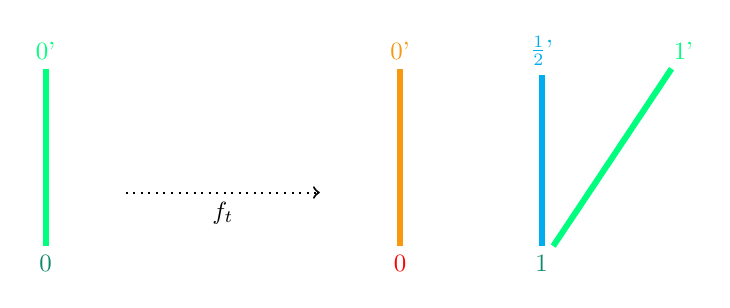
\begin{tikzpicture}[thick,scale=0.9, every node/.style={scale=0.9}]
 		\node (A) at (-2,0) {\textcolor{PineGreen}{0}};
 		\node (B) at (-2,3) {\textcolor{SpringGreen}{0'}};
 		\draw[line width=.03in, SpringGreen] (A) -- (B);
 		
 		\node (C) at (3,0) {\textcolor{red}{0}};
 		\node (D) at (3,3) {\textcolor{YellowOrange}{0'}};
 		\draw[line width=.03in, YellowOrange] (C) -- (D);
 		
 		\node (E) at (5,0) {\textcolor{PineGreen}{1}};
 		\node (F) at (5,3) {\textcolor{cyan}{$\frac{1}{2}$'}};
 		\node (G) at (7,3) {\textcolor{SpringGreen}{1'}};
 		\draw[line width=.03in, cyan] (E) -- (F);
 		\draw[line width=.03in, SpringGreen] (E) -- (G);
 		
 		\node (a) at (-1,1) {};
 		\node (b) at (2,1) {};
 		\draw[->, dotted, line width=.01in] (a) -- node[anchor=north] {$f_{\text{t}}$} (b); 			 	
 	\end{tikzpicture}
 	\caption{$f_t: \textbf{1}_\bot \rightarrow \textbf{1}_\bot + (2\cdot \textbf{1})_\bot$ as $\mathbb{FF_2}$-arrow where $0 \mapsto 1, 0' \mapsto 1'$.}
 \end{figure}
  

 \begin{figure}[h]
 	\centering
 		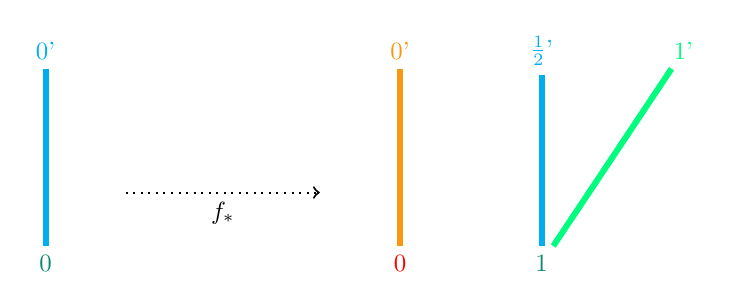
\begin{tikzpicture}[thick,scale=0.9, every node/.style={scale=0.9}]
 		\node (A) at (-2,0) {\textcolor{PineGreen}{0}};
 		\node (B) at (-2,3) {\textcolor{cyan}{0'}};
 		\draw[line width=.03in, cyan] (A) -- (B);
 		
 		\node (C) at (3,0) {\textcolor{red}{0}};
 		\node (D) at (3,3) {\textcolor{YellowOrange}{0'}};
 		\draw[line width=.03in, YellowOrange] (C) -- (D);
 		
 		\node (E) at (5,0) {\textcolor{PineGreen}{1}};
 		\node (F) at (5,3) {\textcolor{cyan}{$\frac{1}{2}$'}};
 		\node (G) at (7,3) {\textcolor{SpringGreen}{1'}};
 		\draw[line width=.03in, cyan] (E) -- (F);
 		\draw[line width=.03in, SpringGreen] (E) -- (G);
 		
 		\node (a) at (-1,1) {};
 		\node (b) at (2,1) {};
 		\draw[->, dotted, line width=.01in] (a) -- node[anchor=north] {$f_{*}$} (b); 			 	
 	\end{tikzpicture}
 	\caption{$f_*: \textbf{1}_\bot \rightarrow \textbf{1}_\bot + (2\cdot \textbf{1})_\bot$ as $\mathbb{FF_2}$-arrow where $0 \mapsto 1, 0' \mapsto \frac{1}{2}'$.}
 \end{figure}
 
 
 \begin{figure}[h]
 	\centering
 		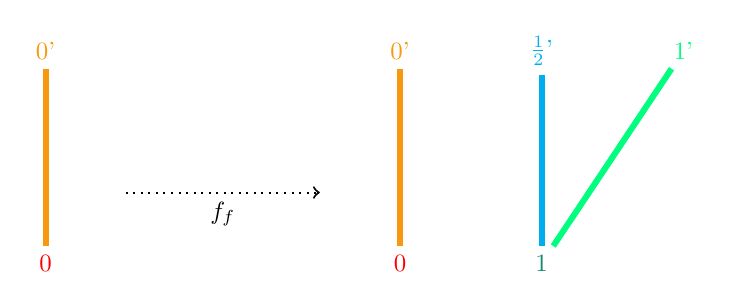
\begin{tikzpicture}[thick,scale=0.9, every node/.style={scale=0.9}]
 		\node (A) at (-2,0) {\textcolor{red}{0}};
 		\node (B) at (-2,3) {\textcolor{YellowOrange}{0'}};
 		\draw[line width=.03in, YellowOrange] (A) -- (B);
 		
 		\node (C) at (3,0) {\textcolor{red}{0}};
 		\node (D) at (3,3) {\textcolor{YellowOrange}{0'}};
 		\draw[line width=.03in, YellowOrange] (C) -- (D);
 		
 		\node (E) at (5,0) {\textcolor{PineGreen}{1}};
 		\node (F) at (5,3) {\textcolor{cyan}{$\frac{1}{2}$'}};
 		\node (G) at (7,3) {\textcolor{SpringGreen}{1'}};
 		\draw[line width=.03in, cyan] (E) -- (F);
 		\draw[line width=.03in, SpringGreen] (E) -- (G);
 		
 		\node (a) at (-1,1) {};
 		\node (b) at (2,1) {};
 		\draw[->, dotted, line width=.01in] (a) -- node[anchor=north] {$f_{\text{f}}$} (b); 			 	
 	\end{tikzpicture}
 	\caption{$f_\text{f}: \textbf{1}_\bot \rightarrow \textbf{1}_\bot + (2\cdot \textbf{1})_\bot$ as $\mathbb{FF_2}$-arrow where $0 \mapsto 0, 0' \mapsto 0$.}
 \end{figure}
 
 
 The objects are translated as follows:
 \begin{itemize}
 	\item At levels $0$ and $1$ the elements of the sets $F_0,F_1$ and $G_0,G_1$ become distinct nodes.
 	\item The transition functions $f: F_0 \rightarrow F_1$ and $g: G_0 \rightarrow G_1$ specify the partial ordering by requiring $\forall_{a\in F_0} \;f(a) \leq a$ and $\forall_{b\in G_0} \;g(b) \leq b$.\newline
 	What we are left with is two finite forests $F$ and $G$. 
 \end{itemize}
 As for the arrows:
 \begin{itemize}
 	\item The natural transformation $\tau: F \Rightarrow G$ in its components $\tau_0,\tau_1$ determines the image of an arrow $f_\tau$ for each node.\newline
 	Notice that the naturality of $\tau$, i.e., $g \tau_0 = \tau_1 f$ makes $f_\tau$ an order-preserving and open map, i.e., an arrow in $\mathbb{FF}$.
 \end{itemize}
 
This method can be generalized from the poset category \textbf{2}, i.e., $0 \xrightarrow{\leq_0} 1$ to a generic functor category of \emph{variable sets}, a.k.a. \emph{finite sets through finite time} $\mathbb{Set}_{fin}^\textbf{N}$ where $\textbf{N}$ is the analogous poset category \textbf{N}, i.e., $0 \xrightarrow{\leq_0} 1 \xrightarrow{\leq_1} 2.. \xrightarrow{\leq_{N-1}} N$ and provides a translation from $\mathbb{Set}_{fin}^\textbf{N}$ to $\mathbb{FF_N}$. \newline
 So:
 \begin{remark}
 	There is a \emph{translation} available from the categories $\mathbb{Set}_{fin}^\textbf{N}$ to the category of finite forests $\mathbb{FF}$. 
 \end{remark} 
 
 At first glance there seems to be a \emph{reverse translation} available from $\mathbb{FF_N}$ to $\mathbb{Set}_{fin}^\textbf{N}$. 
 \newline
 Consider the following example:
 \begin{ex}
 	Let $f: \textbf{1} + \textbf{1}_\bot \times \textbf{1}_\bot \rightarrow \textbf{1}_\bot + (\textbf{1}_\bot)_\bot  $ be an arrow in $\mathbb{FF_3}$:
 	\begin{figure}[h]
 		\centering
 			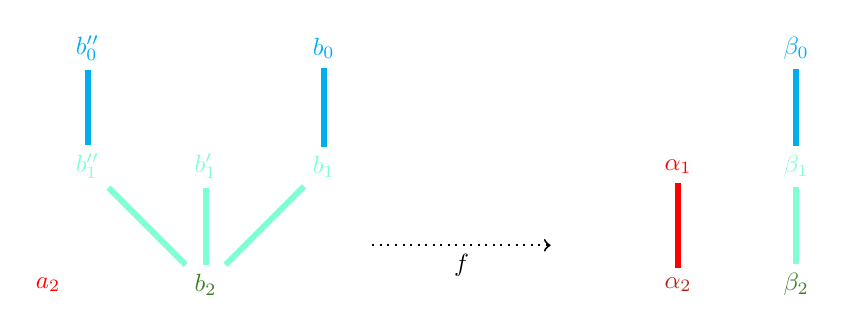
\begin{tikzpicture}[thick,scale=0.5, every node/.style={scale=0.9}]
 				\node (D) at (-2,0) {\textcolor{red}{$a_2$}};
 				
 				\node (F) at (2,0) {\textcolor{OliveGreen}{$b_2$}};
 				\node (G) at (2,3) {\textcolor{Aquamarine}{$b_1'$}};
 				\node (H) at (-1,3) {\textcolor{Aquamarine}{$b_1''$}};
 				\node (I) at (5,3) {\textcolor{Aquamarine}{$b_1$}};
 				\node (J) at (-1,6) {\textcolor{cyan}{$b_0''$}};
 				\node (K) at (5,6) {\textcolor{cyan}{$b_0$}};
 				
 				\node (a) at (6,1) {};
 				\node (b) at (11,1) {};
 				\draw[->, dotted, line width=.01in] (a) -- node[anchor=north] {$f$} (b);
 				
 				\node (L) at (14,0) {\textcolor{BrickRed}{$\alpha_2$}};
 				\node (L') at (14,3) {\textcolor{red}{$\alpha_1$}};
 				
 				\node (M) at (17,0) {\textcolor{OliveGreen}{$\beta_2$}};
 				\node (N) at (17,3) {\textcolor{Aquamarine}{$\beta_1$}};
 				\node (0) at (17,6) {\textcolor{cyan}{$\beta_0$}};
 				
 				\draw[line width=.03in, red] (L) -- (L');
 				\draw[line width=.03in, Aquamarine] (F) -- (G);
 				\draw[line width=.03in, Aquamarine] (F) -- (H);
 				\draw[line width=.03in, Aquamarine] (F) -- (I);
 				\draw[line width=.03in, cyan] (H) -- (J);
 				\draw[line width=.03in, cyan] (I) -- (K);
 				
 				\draw[line width=.03in, Aquamarine] (M) -- (N);
 				\draw[line width=.03in, cyan] (N) -- (0);
 		\end{tikzpicture}
 		\caption{The usual coloring notation is used.\newline So $f: a_2 \mapsto \alpha_2$, $b_1,b_1',b_1'' \mapsto \beta_1$ and $b_0, b_0'' \mapsto \beta_0$.}
 	\end{figure}
 	\newpage
 	If we follow the translation steps in \emph{reverse}, we obtain:
 	
 	\begin{figure}[h]
 		\centering
 		\begin{tikzcd}[scale=0.9]
 			{\{b_0'',} && {b_0\}} &&&& {\{\beta_0} & {\}} \\
 			{\{b_1'',} & {b_1',} & {b_1\}} &&&& {\{\beta_1,} & {\gamma_1\}} \\
 			{\{a_2,} & {b_2} & {\}} &&&& {\{\beta_2,} & {\gamma_2\}}
 			\arrow[maps to, from=1-1, to=2-1]
 			\arrow["{f_0}", maps to, from=1-3, to=2-3]
 			\arrow[maps to, from=2-1, to=3-2]
 			\arrow[maps to, from=2-2, to=3-2]
 			\arrow["{f_1}", maps to, from=2-3, to=3-2]
 			\arrow["{g_0}"', maps to, from=1-7, to=2-7]
 			\arrow["{g_1}"', maps to, from=2-7, to=3-7]
 			\arrow[maps to, from=2-8, to=3-8]
 			\arrow["{\tau_0}"', squiggly, from=1-3, to=1-7]
 			\arrow["{\tau_1}"', squiggly, from=2-3, to=2-7]
 			\arrow["{\tau_2}"', squiggly, from=3-3, to=3-7]
 		\end{tikzcd}
 		\caption{The transition maps are displayed as $F_0 \xrightarrow{f_0} F_1 \xrightarrow{f_1} F_2$ and
 			$G_0 \xrightarrow{g_0} G_1 \xrightarrow{g_1} G_2$}
 	\end{figure}
 	The nodes at each level correspond to sets at a particular time \footnote{in this case either 0,1 or 2.} and the edges between them indicate the transition maps.
 	\newline
 	Notice that, differently from \ref{chapter02}, finite forests seem to \emph{grow} from top to bottom \footnote{the notation reflects this as the top-most nodes have a 0 for subscript} where the transition maps $f_0,f_1$ need not be injective \footnote{this is seen for example with $b_1,b_1',b_1'' \mapsto \beta_1$.} or surjective \footnote{this corresponds for example to the emergence of $b_1' \in F_1$ which is not in the image of $f_0$.}.
 \end{ex}
 

 
 This is reflected in the fact that every transition function from say $F_m$ to $F_n$ with $m \leq n$ is an arbitrary set-function and, as we just said, need not be injective or surjective.\newline
 This simple fact gives the \emph{forest structure} we observed for variable sets. 
 
 \newpage
 The reverse translation from $\mathbb{FF_N}$ to $\mathbb{Set}^\textbf{N}$, however, breaks down when we consider arrows from finite forests of different height like in this simple case:
 
 \begin{ex}
 	Let $!_{\textbf{1}_\bot}$ be the only arrow from $\textbf{1}_\bot$ to the terminal $\textbf{1}$:
 	\begin{figure}[h]
 		\centering
 			\begin{tikzpicture}[thick,scale=0.7, every node/.style={scale=0.9}]
 				\node (A) at (0,0) {\textcolor{orange}{$a_1$}};
 				\node (a) at (0.5,0) {};
 				\node (B) at (0,3) {\textcolor{orange}{$a_0$}};
 				\node (b) at (0.5,3) {};
 				
 				\node (c) at (5.5,0) {};
 				\node (d) at (5.5,0.5) {};
 				\node (C) at (6,0) {\textcolor{orange}{$\alpha_1$}};
 				\draw[line width=.03in, orange] (A) -- (B);
 					\draw[|->, dotted, line width=.01in] (a) -- (c);
 					\draw[|->, dotted, line width=.01in] (b) -- (d);
 			\end{tikzpicture}
 		\caption{$\textbf{1}_\bot \xrightarrow{!_{\textbf{1}_\bot}} \textbf{1}$.}
 	\end{figure}
 	
 	We would need the following to be a commutative diagram:
 	\begin{figure}[h]
 		\centering
 		\begin{tikzcd}
 			& {\{ a_0 \}} && \emptyset \\
 			{} & {\{ a_1 \}} & {} & {\{\alpha_1\}}
 			\arrow["{f_0}", maps to, from=1-2, to=2-2]
 			\arrow["{\tau_1}"', squiggly, from=2-2, to=2-4]
 			\arrow["{g_0= \emptyset_{G_1}}", dashed, maps to, from=1-4, to=2-4]
 			\arrow["{?\tau_0}"', squiggly, from=1-2, to=1-4]
 		\end{tikzcd}
 		\caption{$f_0 : a_0 \mapsto a_1$ and $\tau_1 : a_1 \mapsto \alpha_1$ with $g_0= \emptyset_{G_1}$ the (unique) empty map from $\emptyset$ to $G_1 = \{\beta_1\}$. }
 	\end{figure}
 	\newline
 	But:
 	\begin{remark}
 		There exists no map from a non-empty set like $\{a_0\}$ to the empty-set $\emptyset$ which would be the component $\tau_0$ of $\tau: F \Rightarrow G$.
 	\end{remark}
 \end{ex}
 
 We conclude with the following considerations:
 
 \begin{remark}
 	The \emph{translation} $\tilde{F}$ from $\mathbb{Set}^\textbf{N}$ to $\mathbb{FF_N}$ defines an assignment for objects and morphisms and is functorial.\footnote{the functor $\tilde{F}$ is such that $\tilde{F}(id_A)=id_{\tilde{F}(A)}$ and $F(fg)=F(f)F(g)$.} 
 	\newline
 	The \emph{reverse translation} from $\mathbb{FF_N}$ to $\mathbb{Set}^\textbf{N}$ fails to be an assignment for all $\mathbb{FF_N}$-arrows.
 \end{remark}
 
 
 
 \begin{remark}
 	If, using our imperfect translation, we \emph{compare} the arrows in the two categories one notices for instance that the terminal object in $\mathbb{Set}^\textbf{N}$ is $\{0\} \xrightarrow{id} \{0\} \xrightarrow{id}... \xrightarrow{id}\{0\}$ a.k.a the \emph{finite telephone pole} whilst the terminal object in $\mathbb{FF}_*$ is the singleton forest \textbf{1}. \newline
 	For $N>1$ the \emph{telephone pole} in $\mathbb{FF}_N$, i.e., $((\textbf{1}_{\bot_1})_{\bot_2}..)_{\bot_{N-1}}$ is of course \emph{not} terminal as there can be many distinct arrows into it. \newline
 	Furthermore if we compare the sub-object classifiers (both seen as forests) between $\mathbb{FF_2}$/\emph{bushes} and $\mathbb{Set}^\textbf{2}$ we find a rather different structure:
 \begin{figure}[h]
 	\centering
 	\begin{subfigure}[h]{0.5\textwidth}
 		\centering
 		\begin{tikzcd}
 		{\textcolor{OliveGreen}{\bigcdot}} && \begin{tikzpicture}[scale=0.6]
 			\node (A) at (0,0) {\textcolor{red}{\textbf{f}}};
 			\node (B) at (3,0) {\textcolor{OliveGreen}{\textbf{t}}};
 			\node (C) at (3,3) {\textcolor{cyan}{$*$}};
 			\draw[cyan, line width=.03in] (B) -- (C);
 		\end{tikzpicture}
 		\arrow["true", from=1-1, to=1-3]
 	\end{tikzcd}
 	\caption{$\top : \mathbf{1} \xrightarrow{true} (\textbf{1} + \textbf{1}_\bot)$.}
 	\end{subfigure}
 	\hfil
 	\centering
 	\begin{subfigure}[h]{0.5\textwidth}
 		\centering
		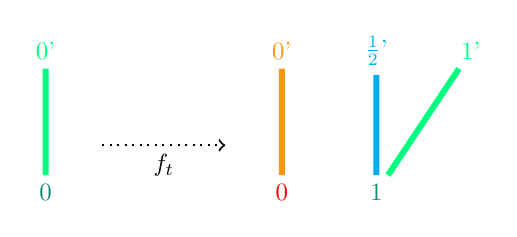
\begin{tikzpicture}[thick,scale=0.6, every node/.style={scale=0.9}]
			\node (A) at (-2,0) {\textcolor{PineGreen}{0}};
			\node (B) at (-2,3) {\textcolor{SpringGreen}{0'}};
			\draw[line width=.03in, SpringGreen] (A) -- (B);
			
			\node (C) at (3,0) {\textcolor{red}{0}};
			\node (D) at (3,3) {\textcolor{YellowOrange}{0'}};
			\draw[line width=.03in, YellowOrange] (C) -- (D);
			
			\node (E) at (5,0) {\textcolor{PineGreen}{1}};
			\node (F) at (5,3) {\textcolor{cyan}{$\frac{1}{2}$'}};
			\node (G) at (7,3) {\textcolor{SpringGreen}{1'}};
			\draw[line width=.03in, cyan] (E) -- (F);
			\draw[line width=.03in, SpringGreen] (E) -- (G);
			
			\node (a) at (-1,1) {};
			\node (b) at (2,1) {};
			\draw[->, dotted, line width=.01in] (a) -- node[anchor=north] {$f_{\text{t}}$} (b); 			 	
		\end{tikzpicture}
		\caption{$f_t: \textbf{1}_\bot \rightarrow \textbf{1}_\bot + (2\cdot \textbf{1})_\bot$.}
 	\end{subfigure}
 \end{figure}
 \end{remark}

 	We conclude with the following observation:
%check 	
 	\begin{remark}
 		Having fixed an $N>0$, the arrows in $\mathbb{FF}_N$ that can be translated into natural transformations in $\mathbb{Set}^\textbf{N}$ must have the following requirements:
 		\begin{itemize}
 			\item the finite forests in the domain and co-domain must have the same height equal to $N$.
 			\item each node must be sent to a node of equal height. 
 		\end{itemize}
 	\end{remark}
 	
 	In a nutshell, for $N > 1$: 
 	
 	\begin{remark}
 		There are \emph{more} arrows in $\mathbb{FF}_N$ than in $\mathbb{Set}^\textbf{N}$.	
 	\end{remark}
 	
 	     
\begin{remark}
	Though remarkably similar, for any $N>0$ the categories of \emph{Variable Finite Sets} $\mathbb{Set}^\textbf{N}$ and \emph{finite forests of height at most N} $\mathbb{FF}_N$ in fact have very different structures.
	\newline
	The most relevant distinction for our concerns is that: $\mathbb{Set}^\textbf{N}$ is a topos for all $N$, while $\mathbb{FF}_N$, as we have proven through the lengthy counterexample in \ref{counterex},  is a topos only for $N \leq 2$.
\end{remark}
 
 	\newpage
 ${}$ \newpage